% Este archivo es ejemplo-articulo-regular-es.tex, un capítulo
% de ejemplo (en español) del paquete 'sistedes' para la
% Biblioteca Digital de Sistedes; Version 1.0 de 07/02/2023
%
% Este paquete extiende el paquete LLNCS de Springer Computer
% Science proceedings.
\documentclass[runningheads]{sistedes}

\usepackage[spanish,es-tabla]{babel}

\usepackage{graphicx}
% Usado para mostrar la figura de ejemplo. 
%
% Si usa el paquete hyperref, elimine los comentarios de las
% siguientes dos líneas para mostrar las URLs en fuente romana
% azul de acuerdo con el estilo del libro electrónico de Springer:
%\usepackage{color}
%\renewcommand\UrlFont{\color{blue}\rmfamily}
%
\begin{document}
%
\title{Título de la contribución\thanks{Financiado por la organización x.}}
%
%\titlerunning{Título abreviado}
% Si el título del artículo es demasiado largo para el encabezado,
% puede establecer un título de artículo abreviado aquí
%
\author{Primer Autor\inst{1}\orcidID{0000-1111-2222-3333} \and
Segundo Autor\inst{2,3}\orcidID{1111-2222-3333-4444} \and
Tercer Autor\inst{3}\orcidID{2222--3333-4444-5555}}
%
\authorrunning{F. Autor et al.}
% Los nombres se abrevian en el encabezado.
% Si hay más de dos autores, se usa 'et al.'
%
\institute{Princeton University, Princeton NJ 08544, USA \and
Springer Heidelberg, Tiergartenstr. 17, 69121 Heidelberg, Germany
\email{lncs@springer.com}\\
\url{http://www.springer.com/gp/computer-science/lncs} \and
ABC Institute, Rupert-Karls-University Heidelberg, Heidelberg, Germany\\
\email{\{abc,lncs\}@uni-heidelberg.de}}
%
\maketitle              % Componer el encabezado de la contribución
%
\begin{abstract}
El resumen debe resumir brevemente el contenido del trabajo en
150--250 palabras.

\keywords{primera palabra clave  \and segunda palabra clave \and
otra palabra clave.}
\end{abstract}
%
%
%
\section{Primera sección}
\subsection{Subsección de muestra}
Todos los párrafos se indentan, acorde a la configuración en español 
proporcionada por el paquete \verb|babel|.

\subsubsection{Encabezado de muestra (Tercer nivel)}
Solo se deben numerar dos niveles de encabezados. Los encabezados de nivel
inferior permanecen sin numerar; y se colocan en la misma línea que el texto
que los sigue.

\paragraph{Encabezado de muestra (Cuarto nivel)}
La contribución no debe contener más de cuatro niveles de encabezados.
La Tabla~\ref{tab1} muestra un resumen de todos los niveles de encabezado.

\begin{table}
\caption{Los títulos de las tablas deben colocarse arriba.}\label{tab1}
\begin{tabular}{|l|l|l|}
\hline
Nivel de encabezado & Ejemplo & Tamaño y estilo\\
\hline
Título (centrado) &  {\Large\bfseries Lecture Notes} & 14 puntos, negrita\\
Encabezado nivel 1 &  {\large\bfseries 1 Introduction} & 12 puntos, negrita\\
Encabezado nivel 2 & {\bfseries 2.1 Printing Area} & 10 puntos, negrita\\
Encabezado nivel 3 & {\bfseries Run-in Heading in Bold.} Texto a continuación & 10 puntos, negrita\\
Encabezado nivel 4 & {\itshape Lowest Level Heading.} Texto a continuación & 10 puntos, cursiva\\
\hline
\end{tabular}
\end{table}


Las ecuaciones se mostrarán centradas y en una línea separada.

\begin{equation}
x + y = z
\end{equation}
Intente evitar imágenes rasterizadas para diagramas, figuras y gráficas. 
Siempre que sea posible, utilice gráficos vectoriales en su lugar
(ver Fig.~\ref{fig1}).

\begin{figure}
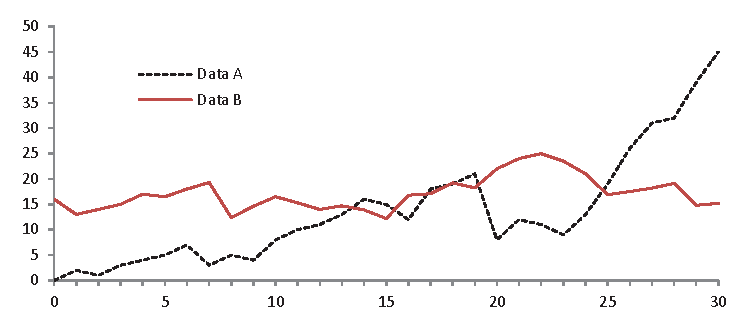
\includegraphics[width=\textwidth]{fig1.eps}
\caption{Los pies de figura siempre se coloca debajo de la ilustración.
Tenga en cuenta que los subtítulos cortos están centrados, mientras que
los largos se mostrarán justificados de forma automática.} \label{fig1}
\end{figure}

\begin{theorem}
Este es un teorema de muestra. El título inicial está en negrita, mientras
que el siguiente texto aparece en cursiva. Las definiciones, los lemas,
las proposiciones y los corolarios se mostrarán con un  mismo estilo similar.
\end{theorem}
%
% Los entornos 'definition', 'lemma', 'proposition', 'corollary',
% 'remark', and 'example' se definen en la clase LLNCS de LaTeX.
%
\begin{proof}
Las demostraciones, ejemplos y acotaciones tienen la palabra inicial en cursiva,
mientras que el resto del texto aparece en tipografía romana.
\end{proof}
Para las citas de referencias, se prefiere el uso de corchetes
y números consecutivos. Citas con etiquetas o autor/año también
son aceptables. La siguiente bibliografía proporciona una lista de referencias
de muestra con entradas para artículos de revistas~\cite{ref_article1},
un capítulo de LNCS~\cite{ref_lncs1}, un libro~\cite{ref_book1},
actas sin editores~\cite{ref_proc1}, y una página de inicio~\cite{ref_url1}.
Las citas múltiples se han de agrupar
\cite{ref_article1,ref_lncs1,ref_book1},
\cite{ref_article1,ref_book1,ref_proc1,ref_url1}.

\subsubsection{Agradecimientos} Coloque sus agradecimientos al final del
artículo, precedido por un encabezado no numerado (es decir, encabezamiento
de 3er nivel).

%
% ---- Bibliografía ----
%
% Los usuarios de BibTeX deben especificar el estilo de bibliografía 'splncs04'.
% Las referencias se ordenarán y formatearán con el estilo correcto.
%
% \bibliographystyle{splncs04}
% \bibliography{mybibliography}
%
\begin{thebibliography}{8}
\bibitem{ref_article1}
Author, F.: Article title. Journal \textbf{2}(5), 99--110 (2016)

\bibitem{ref_lncs1}
Author, F., Author, S.: Title of a proceedings paper. In: Editor,
F., Editor, S. (eds.) CONFERENCE 2016, LNCS, vol. 9999, pp. 1--13.
Springer, Heidelberg (2016). \doi{10.10007/1234567890}

\bibitem{ref_book1}
Author, F., Author, S., Author, T.: Book title. 2nd edn. Publisher,
Location (1999)

\bibitem{ref_proc1}
Author, A.-B.: Contribution title. In: 9th International Proceedings
on Proceedings, pp. 1--2. Publisher, Location (2010)

\bibitem{ref_url1}
LNCS Homepage, \url{http://www.springer.com/lncs}. Last accessed 4
Oct 2017
\end{thebibliography}
\end{document}
